\documentclass{standalone}
\usepackage{tikz}

\begin{document}
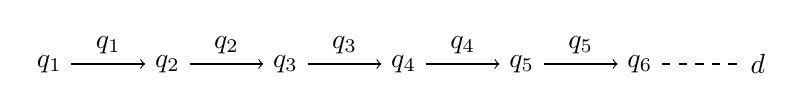
\begin{tikzpicture}[node distance=2cm]
    % Define nodes for each patch
    \foreach \i in {1,...,6} {
        \node (patch\i) at (\i*1.5,0) {$q_{\i}$};
    }

    % Draw arrows between patches
    \draw[->] (patch1) -- node[midway, above]{$q_1$} (patch2);
    \draw[->] (patch2) -- node[midway, above]{$q_2$} (patch3);
    \draw[->] (patch3) -- node[midway, above]{$q_3$} (patch4);
    \draw[->] (patch4) -- node[midway, above]{$q_4$} (patch5);
    \draw[->] (patch5) -- node[midway, above]{$q_5$} (patch6);

    % Add random movement rate as a dashed line
    \draw[dashed] (patch6.east) -- ++(1,0) node[right]{$d$};

\end{tikzpicture}
\end{document}